\documentclass[openany]{amsbook}

\usepackage[a5paper,margin=28mm,marginparwidth=20mm,marginparsep=3mm]{geometry}
\usepackage{verse,microtype,mathtools,xfrac,marginnote,graphicx,ragged2e,xstring,afterpage,pifont}

\usepackage{fontspec}
\usepackage[T1]{fontenc}
\newfontfamily\hoskeroe{English Towne}
\newfontfamily\greekish{CMU Serif}
\newfontfamily\arabicish{KacstQurn}
\newfontfamily\frakturish{Fette UNZ Fraktur}
\setmainfont[Numbers=OldStyle]{Latin Modern Roman}
\newfontfamily\scshape[Letters=SmallCaps]{Latin Modern Roman Caps}

\usepackage[hidelinks]{hyperref}

\newcommand{\poeticmarginnote}[1]{\marginnote{\footnotesize #1}}

\newcommand\blfootnote[1]{%
  \begingroup
  \renewcommand\thefootnote{}\footnote{#1}%
  \addtocounter{footnote}{-1}%
  \endgroup
}

\title{The Second Book}

\begin{document}
\frontmatter
\maketitle

\thispagestyle{empty}
\topskip0pt
\vspace*{\fill}
\noindent {\it And the great dragon was thrown down, that ancient serpent, who is called the Devil and Satan, the deceiver of the whole world -- he was thrown down to the earth, and his angels were thrown down with him. And I heard a loud voice in heaven, saying, Now the salvation and the power and the kingdom of our God and the authority of his Christ have come, for the accuser of our brethren has been thrown down, who accuses them day and night before our God... But woe to you, O earth and sea, for the devil has come down to you in great wrath, because he knows that his time is short...}
\vspace*{\fill}
\clearpage

\tableofcontents

\thispagestyle{empty}
\topskip0pt
\vspace*{\fill}
{\centering
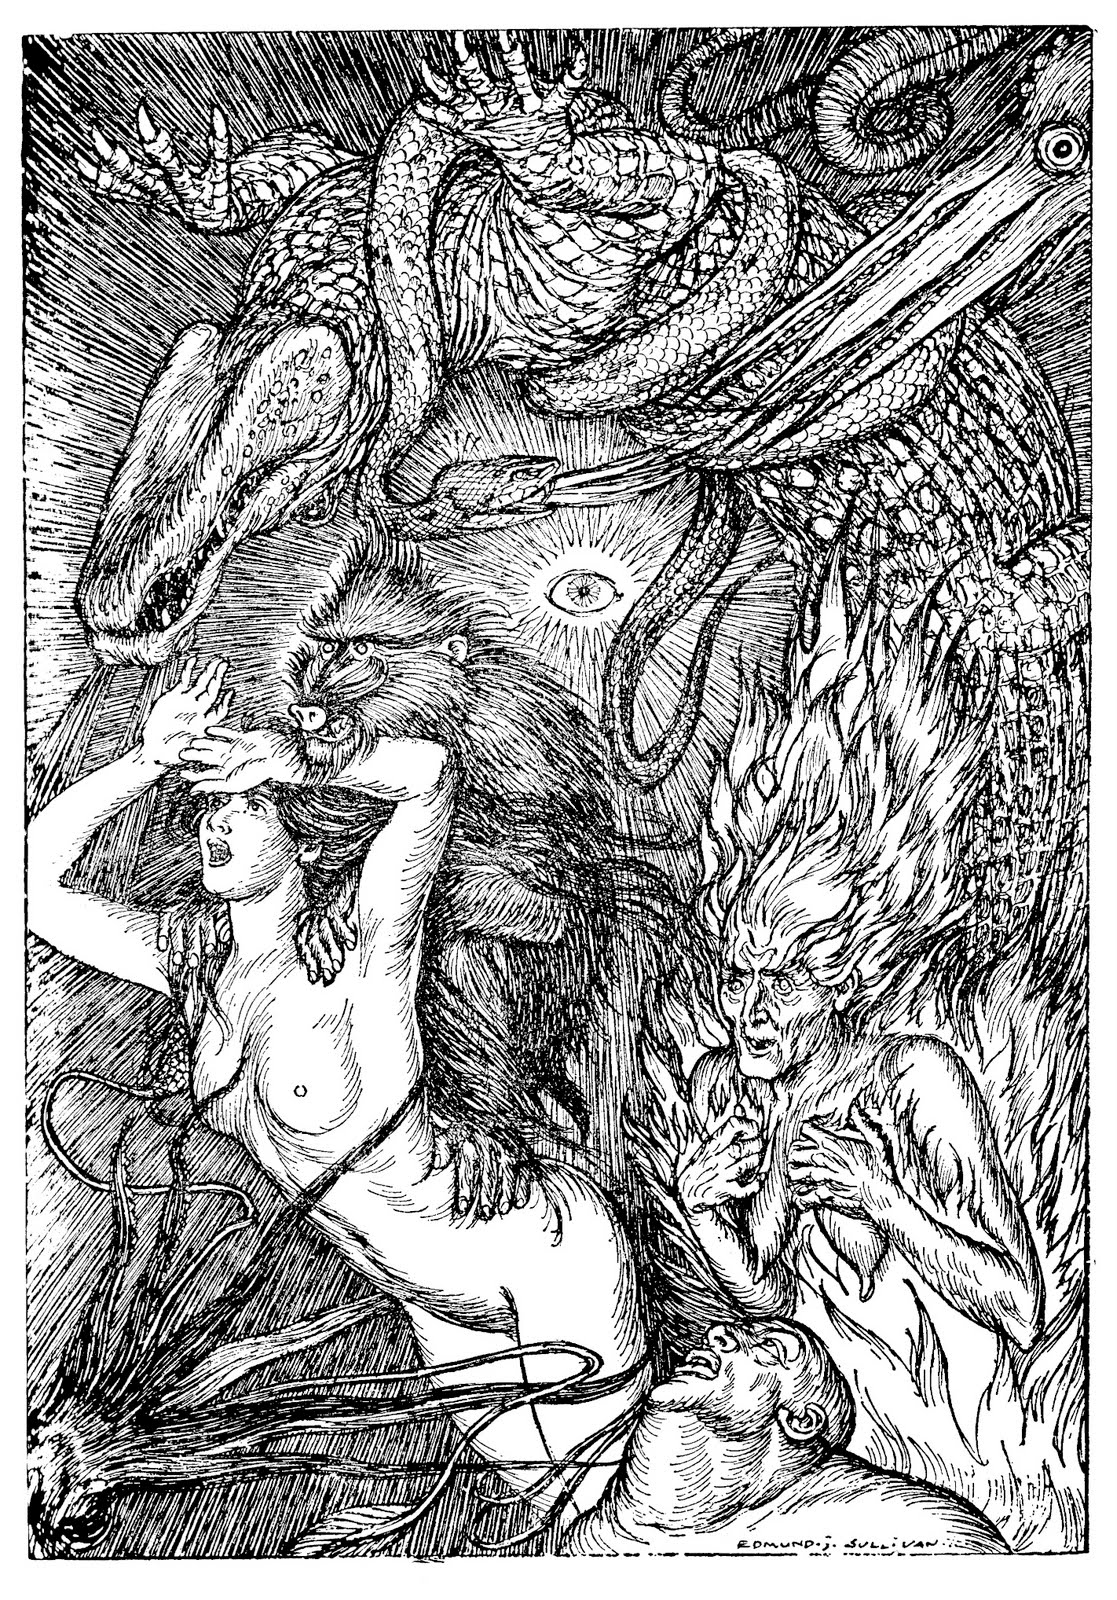
\includegraphics[width=\textwidth]{images/placeholder_image.jpg}}
\vspace*{\fill}
\clearpage

\mainmatter

#THE_POEMS

\bigskip
\bigskip
\begin{center}
\textsc{End of the Second Book}
\end{center}

\end{document}
